\section{The Empirical Dust Attenuation Framework} \label{sec:dem}
\chedit{
    In this section, we describe the Empirical Dust Attenuation (\eda)
    framework and present the \eda~prescription we use in this work. 
    The \eda~is a flexible framework for applying dust attenuation curves to
    simulated galaxy populations.
    For each simulated galaxy, the \eda~assigns a dust attenuation
    curve that is parameterized as a function of the galaxy's properties 
    ($M_*$, ${\rm SSFR}$), the \eda~parameters, and randomly
    sampled inclination. With the \eda, we can apply a wide variety of dust
    attenuation that include correlation between dust attenuation and physical
    galaxy properties. 
}
% Later, we demonstrate that we can accurately reproduce SDSS observations with the \eda~and use it to test galaxy formation models and shed light on dust in galaxies. 

We begin by defining the dust attenuation curve, $A(\lambda)$, as 
\begin{equation} \label{eq:full_atten}
    F_o (\lambda) = F_i (\lambda) 10^{-0.4 A(\lambda)}
\end{equation}
where $F_o$ is the observed flux and $F_i$ is the intrinsic flux. We normalize
the attenuation to the $V$ band attenuation, 
\begin{equation} 
    A(\lambda) = A_V \frac{k(\lambda)}{k_V}
\end{equation}
so that $A_V$ determines the amplitude of the attenuation, while $k(\lambda)$
determines the wavelength dependence. 

\chedit{
    The \eda~framework assigns $A(\lambda)$ to every galaxy in the simulations
    using some flexible prescription. For the \eda~prescription in this work,
    we assign $A_V$ for each galaxy using the slab model, where $A_V$ is a
    function of galaxy inclination, $i$, and its optical depth,
    $\tau_V$~\citep[\eg][]{somerville1999, somerville2012}: 
}
\begin{equation} \label{eq:slab}
    A_V = -2.5 \log \left[ \frac{1 - e^{-\tau_V\,\sec i}}{\tau_V\,\sec i} \right].
\end{equation}
We parameterize $\tau_V$ using a linear $M_*$ and $\ssfr$ dependence: 
\begin{equation} \label{eq:tauv}
    \tau_V(M_*, \sfr) = \mtaum \log \left(\frac{M_*}{10^{10} M_\odot}\right) +
    \mtaus \log \left(\frac{\ssfr}{10^{-10}yr^{-1}}\right) + c_\tau.
\end{equation}
$\mtaum$, $\mtaus$, and $c_\tau$ represent the $M_*$ dependence, the $\ssfr$
dependence, and amplitude of $\tau_V$. Since $\tau_V$ is optical depth, we
impose a $\tau_V \ge 0$ limit.
For each galaxy, we uniformly sample $\cos i$ from 0 to 1. By sampling
$\cos i$, our \eda~prescription includes significant variance in
$A(\lambda)$ so galaxies with the same galaxy properties do not have the
same dust attenuation.

\chedit{
    Previous works, motivated by the fact that dust on small scales depend on
    local stellar and gas properties, have parameterized dust attenuation based
    on galaxy properties such as its gas density, gas metallicity, or star-gas
    geometry~\citep[\eg][]{somerville1999, somerville2012, steinacker2013,
    camps2015, narayanan2018, trayford2020, vogelsberger2020}. 
    The galaxies in the SIMBA, TNG, and EAGLE simulations, however, have
    substantially different gas masses and metallicites~\citep[][Maller \etal~in prep.]{dave2020}.  
    If we were to parameterize $\tau_V$ using these properties, the differences
    in them between the simulations would dominate any comparison of dust attenation.
    Instead, we parameterize $\tau_V$ on correlation between dust attenuation
    and galaxy properties that have been established in observations~\citep[\eg~][]{garn2010, battisti2016, salim2020}.
    In Appendix~\ref{sec:slab}, we confirm the correlation between $A_V$ and
    the properties $M_*$ and $\ssfr$ using the \cite{salim2018} GSWLC2 sample
    (Figure~\ref{fig:dep}). 
    We therefore include in Eq.~\ref{eq:tauv} the correlation between $A_V$ and
    galaxy $M_*$ and $\ssfr$.
}


%\tksedit{
%The true properties of dust (grain size, temperature, and spatial
%distributions), determined by detailed dust growth and destruction processes,
%depend on local stellar and gas properties and the local star, gas, and dust
%geometries. 
%On scales relative for large-scale simulations the dust properties
%are expected to vary with gas density (alternatively gas column density or
%total gas mass), gas metallicity, and the relative star-gas geometry, and this
%is often used in estimations of attenuation of starlight by dust
%\citep[e.g.][]{somerville1999, somerville2012, steinacker2013, camps2015,
%narayanan2018, trayford2020, vogelsberger2020}.
%In this work we take an
%observation-centered approach to modeling dust and therefore base our model on
%observationally found relations between galaxy properties, $M_*$ and $\ssfr$,
%and dust attenuation. Moreover, the galaxy populations in the SIMBA, TNG, and
%EAGLE simulations show a variety of distributions in gas mass and gas
%metallicity which would dominate any inference we could make on the relation
%between dust and the galaxy population (e.g. \citealp{dave2020}, Maller et al.
%in prep.). We will explore the relation between our inferred attenuation and
%gas properties and compare in future work (Starkenburg et al. in prep.).
%}

\chedit{
    In Eq.~\ref{eq:slab}, we use the slab model because it provides a simple
    prescription for generating a distribution of $A_V$ that depends on
    randomly sampled $i$, with loose physical motivations.
    For star-forming galaxies, which typically have disc-like morphologies, the
    slab model produces $A_V$ that is correlated with $i$ in a way consistent
    with observations: edge-on galaxies have higher $A_V$ than face-on
    galaxies~\citep[\eg][]{conroy2010, wild2011, battisti2017, salim2020}.
    Nevertheless, the slab model is a naive approximation; in reality, $A_V$
    depends on the detailed star-to-dust geometry.
    Furthermore, all galaxies in the simulations are assigned $A_V$ from the
    slab model.
    For quiescent galaxies, which typically have elliptical morphologies, the
    slab model serves only as an \emph{empirical} prescription for statistically 
    sampling $A_V$. 
    However, the purpose of the~\eda~is to assign an accurate distribution of dust
    attenuation curves for the galaxy population --- \emph{not} to accurately
    model dust attenuation for individual galaxies.
    In this regard, we demonstrate that the slab model based \eda~can match the
    observed distribution of $A_V$, even for samples that include quiescent
    galaxies (Appendix~\ref{sec:slab}).
    Hence, the slab model provides a sufficient prescription for reproducing
    the $A_V$ distribution for all galaxies. 
}

For the wavelength dependence of the attenuation curve, $k(\lambda)$, we
use the \cite{noll2009} parameterization: 
\begin{equation} \label{eq:noll}
    k(\lambda) = \left(k_{\rm Cal}(\lambda) + D(\lambda)\right) \left(
    \frac{\lambda}{\lambda_V} \right)^\delta.
\end{equation}
Here $k_{\rm Cal}(\lambda)$ is the \cite{calzetti2001} curve: 
\[
    k_{\rm Cal}(\lambda) = 
    \begin{cases} 
        2.659 (-1.857 + 1.040/\lambda) + R_V, & 6300 A \le \lambda \le
        22000 A \\ 
        2.659 (-2.156 + 1.509/\lambda - 0.198/\lambda^2 + 0.011/\lambda^3) +
        R_V & 1200 A \le \lambda \le 6300 A
    \end{cases}
\]
where $\lambda_V = 5500 A$ is the $V$ band wavelength and $\delta$ is the slope
offset of the attenuation curve from $k_{\rm Cal}$. Since $\delta$ correlates 
with galaxy properties~\citep[\eg][; see also Appendix~\ref{sec:slab}]{wild2011, battisti2016, leja2017, salim2018},
we parameterize $\delta$ with a similar $M_*$ and $\ssfr$ dependence as
$\tau_V$:  
\begin{align} \label{eq:delta}
    \delta(M_*, \sfr) &= \mdeltam \log \left(\frac{M_*}{10^{10}
    M_\odot}\right) + \mdeltas \log \left(\frac{\ssfr}{10^{-10}yr^{-1}}\right)
    + c_\delta.
\end{align}
% Although a number of works have found correlation between the attenuation
% curve slope and inclination~\citep{wild2011, chevallard2013, battisti2017b},
% \cite{salim2020}, most recently, found that the driver of this trend is the
% relationship between $A_V$ and slope. We therefore do not include an
% inclination dependence in $\delta$. 
$D(\lambda)$ in Eq.~\ref{eq:noll} is the UV dust bump, which we parameter using
the standard Lorentzian-like Drude profile:
\begin{equation}
    D(\lambda) = \frac{E_b(\lambda~\Delta \lambda)^2}{(\lambda^2 -
    \lambda_0^2)^2 + (\lambda~\Delta \lambda)^2}
\end{equation}
where $\lambda_0$, $\Delta \lambda$, and $E_b$ are the central wavelength,
full width at half maximum, and strength of the bump, respectively. 
\chedit{
    We include the UV dust bump since we use UV color as one of our observables.
}
We assume fixed $\lambda_0 = 2175
A$ and $\Delta \lambda = 350A$. \cite{kriek2013} and \cite{tress2018} find
that $E_b$ correlates with the $\delta$ for star-forming galaxies $z\sim2$.
\cite{narayanan2018} confirmed this dependence in simulations. 
However, we assume a fixed relation between $E_B$ and $\delta$ from
\cite{kriek2013}: $E_b = -1.9~\delta + 0.85$. Allowing the slope and amplitude
of the $E_B$ and $\delta$ relation to vary does {\em not} impact our results;
however, we also do not derive any meaningful constraints on them. In
Table~\ref{tab:free_param}, we list and describe all of the free parameters of
the \eda. 

%In $\tau_V$ we include the correlation between $A_V$ and the galaxy's properties , found in both observations and simulations~\citep[\eg][]{narayanan2018, salim2020}. 


$\ssfr$ of galaxies are used to calculate $\tau_V$ and $\delta$ in
Eqs.~\ref{eq:tauv} and~\ref{eq:delta}. However, due to mass and temporal resolutions,
some galaxies in the simulations have $\sfr=0$ --- \ie~an unmeasurably low
SFR~\citep{hahn2019c}. They account for 17, 19, 9\% of galaxies
in SIMBA, TNG, and EAGLE, respectively. Since Eqs.~\ref{eq:tauv}
and~\ref{eq:delta} depend on $\log\ssfr$, they cannot be used in the equations
to derive $\tau_V$ and $\delta$ for these galaxies. To account for this issue,
we assign $\sfr_{\rm min}$, the minimum non-zero $\sfr$ in the simulations, to
$\sfr=0$ galaxies when calculating $\tau_V$ and $\delta$. For SIMBA, TNG, and
EAGLE, $\sfr_{\rm min}=0.000816$, $0.000268$, and $0.000707 M_\odot/yr$. Although 
this assumes that $\sfr=0$ galaxies have similar dust properties as the galaxies 
with $\sfr = \sfr_{\rm min}$, since the simulations have very low $\sfr_{\rm min}$ 
we expect galaxies with $\sfr = \sfr_{\rm min}$ to have little recent
star-formation and low gas mass, similar to $\sfr=0$ galaxies. 

%Since $\sfr=0$ galaxies do not account for a large fraction of our simulated galaxies, we directly sample their observables ($G, R, NUV$, and $FUV$) from the distribution of observables for SDSS quiescent galaxies. This way, we ensure that the attenuation of $\sfr=0$ galaxies does not impact the rest of the \eda~parameters. In Appendix~\ref{sec:res}, we discuss the resolution effects in more detail and demonstrate that our results are \emph{not} impacted by other prescriptions for attenuating $\sfr=0$ galaxies.

\chedit{
    In practice, to apply the \eda~to a simulated galaxy population, we first
    assign a randomly sampled $i$ to each galaxy ($\cos i$ uniformly sampled from 0 to 1).
    $\tau_V$ and $\delta$ are calculated for
    the galaxy based on its $M_*$,
    $\ssfr$ and the \eda~parameters. We then combine $A_V$ from $i$ and
    $\tau_V$ with $k(\lambda)$ from $\delta$ to determine $A(\lambda)$ for each
    galaxy.
} 
Afterwards, we attenuate the galaxy SEDs using Eq.~\ref{eq:full_atten} and use
the attenuated SEDs to calculate the observables: $g, r, NUV$, and $FUV$
absolute magnitudes. 
\ch{
    In Figure~\ref{fig:dem_av}, we present attenuation curves, $A(\lambda)$,
    generated by the \eda~for galaxies with different $\sfr$ and $M_*$ values.  
    We include star-forming galaxies with $\{M_*, \sfr\} = \{10^{10}M_\odot,
    10^{0.5}M_\odot/yr\}$ (blue), $\{10^{11}M_\odot, 10^{1} M_\odot/yr\}$
    (green) and a quiescent galaxy with $\{10^{11}M_\odot, 10^{-2}M_\odot/yr\}$
    (red).
    We use an arbitrarily set of \eda~parameters ($\mtaum, \mtaus, c_\tau,
    \mdeltam, \mdeltas, c_\delta$) within the prior range listed in
    Table~\ref{tab:free_param}. 
    We set $i=0$ (edge-on) for all $A(\lambda)$ in Figure~\ref{fig:dem_av} for
    simplicity.
    In practice the \eda~uniformly samples $\cos i$ from 0 to 1 for each galaxy.
}
For comparison, we include the \cite{calzetti2001} attenuation curve. Even when
we set $i=0$, the \eda~produces attenuation curves with a wide range
of amplitude and slope to galaxies based on their physical properties. 

\begin{figure}
\begin{center}
    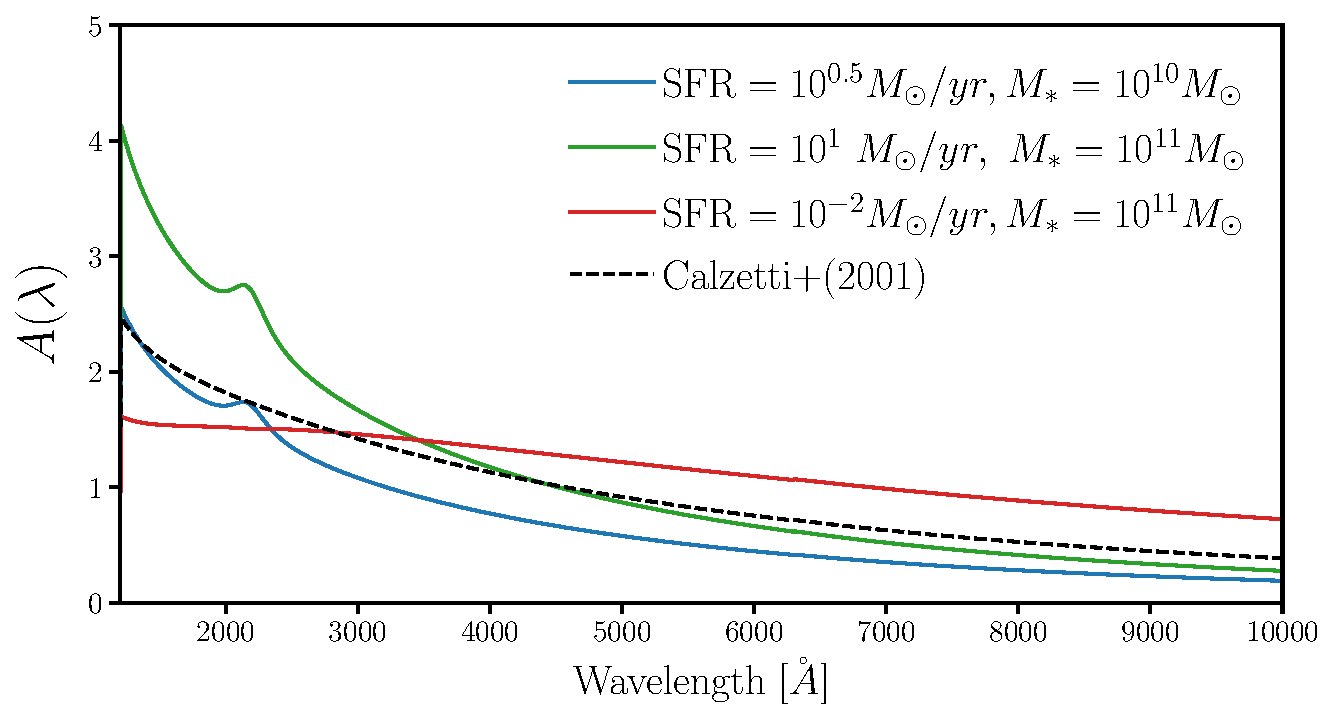
\includegraphics[width=0.6\textwidth]{figs/dems.pdf}
    \caption{\label{fig:dem_av}
    \chedit{
        Attenuation curves, $A(\lambda)$, assigned by our Empirical Dust
        Attenuation (\eda) prescription to edge-on galaxies with different $\sfr$ and
        $M_*$ values for an arbitrary set of \eda~parameters. We include
        $A(\lambda)$ for star-forming galaxies with $\{M_*, \sfr\} =
        \{10^{10}M_\odot, 10^{0.5}M_\odot/yr\}$ (blue), $\{10^{11}M_\odot, 10^{1}
        M_\odot/yr\}$ (green) and a quiescent galaxy with $\{10^{11}M_\odot,
        10^{-2}M_\odot/yr\}$ (red). We set $i=0$ for
        all the galaxies in the figure for simplicity but in practice the
        \eda~uniformly samples $\cos i$ from 0 to 1 for each galaxy.
        For comparison, we include the \cite{calzetti2001} attenuation curve.
        {\em The \eda~provides a flexible prescription for assigning dust
        attenuation to galaxies based on their inclination, physical properties
        ($M_*$ and $\ssfr$), and the \eda~parameters.}
    }
    } 
\end{center}
\end{figure}


%%%%%%%%%%%%%%%%%%%%%%%%%%%%%%%%%%%%%%%%%%
% table of free parameters
%%%%%%%%%%%%%%%%%%%%%%%%%%%%%%%%%%%%%%%%%%
\begin{table}
    \caption{Free parameters of the Empirical Dust Attenuation Model}
    \begin{center}
        \begin{tabular}{ccc} \toprule
            Parameter & Definition & prior\\[3pt] \hline\hline
            %\multicolumn{3}{c}{DEM with slab model}\\ \hline
            $\mtaum$ & $M_*$ dependence of the optical depth, $\tau_V$ & flat $[-5., 5.]$\\
            $\mtaus$ & $\ssfr$ dependence of $\tau_V$  & flat $[-5., 5.]$\\
            $c_{\tau}$ & amplitude of $\tau_V$ & flat $[0., 6.]$\\
            %\hline
            %\multicolumn{3}{c}{DEM with $\mathcal{N}_T$ model}\\ \hline
            %$m_{\mu,1}$ & Slope of the $\log M_*$ dependence of optical depth,
            %$\tau_V$ & flat $[-5., 5.]$\\
            %$m_{\mu,2}$ & Slope of the $\log {\rm SFR}$ dependence of optical
            %depth, $\tau_V$ & flat $[-5., 5.]$\\
            %$c_{\mu}$ & amplitude of the optical depth, $\tau_V$ & flat $[0., 6.]$\\ 
            %$m_{\sigma,1}$ & Slope of the $\log M_*$ dependence of optical depth, $\tau_V$ & flat $[-5., 5.]$\\
            %$m_{\sigma,2}$ & Slope of the $\log {\rm SFR}$ dependence of optical depth, $\tau_V$ & flat $[-5., 5.]$\\
            %$c_{\sigma}$ & amplitude of the optical depth, $\tau_V$ & flat $[0.1, 3.]$\\ 
            %\hline
            $\mdeltam$ & $M_*$ dependence of $\delta$, the attenuation curve slope offset & flat $[-4., 4.]$\\
            $\mdeltas$ & $\ssfr$ dependence of $\delta$ & flat $[-4., 4.]$\\
            $c_{\delta}$ & amplitude of $\delta$ & flat $[-4., 4.]$\\
            %$f_{\rm neb}$ & nebular attenuation fraction & flat $[1., 4.]$\\
            \hline
        \end{tabular} \label{tab:free_param}
    \end{center}
\end{table}
%%%%%%%%%%%%%%%%%%%%%%%%%%%%%%%%%%%%%%%%%%

